\section{Evaluation}
\label{sec:evaluation}

\subsection{Experimental Setup}
We evaluate LLaMA2-7B on the WikiText-2 test split using a non-overlapping 2048-token protocol (166 blocks, 339{,}802 loss tokens).
Fake-quantized weights and activations are dequantized before \texttt{F.linear}; attention internals, LayerNorm, and \texttt{lm\_head} remain in FP16 unless noted.
Group size is G16 for the primary design point.
BiE-family outlier detection uses $\mathrm{threshold}(X) = \mathrm{mean}(X) + 3\,\mathrm{std}(X)$ over signed tensor values.

\subsection{Accuracy Results}
Table~\ref{tab:ppl} compares representative quantization formats against an FP16 reference.
Activation-only BiE and Top-2 capping recover most of the accuracy gap of vanilla BFP4 while keeping weights in lower-cost single-exponent BFP.

\begin{table}[t]
    \centering
    \caption{WikiText-2 perplexity on LLaMA2-7B (G16, BFP4/BiE4 family).}
    \label{tab:ppl}
    \begin{tabular}{lc}
        \toprule
        Configuration & PPL \\
        \midrule
        FP16 baseline & 5.472 \\
        Vanilla W/A-BFP4 & 6.283 \\
        W/A-BiE4 & 5.974 \\
        W-BFP4 / A-BiE4 & 6.013 \\
        W-BFP4 / Top-2 A-BiE4 & 6.016 \\
        \bottomrule
    \end{tabular}
\end{table}

\subsection{DEWA Threshold Sweep}
Fig.~\ref{fig:hybrid_sweep} shows perplexity sensitivity to asymmetric DEWA thresholds under W-BFP4 / Top-2 A-BiE4.
A wide operating region near the Top-2 baseline PPL (6.016) indicates that aggressive FP-Acc bypassing is compatible with negligible accuracy loss.

\begin{figure}[t]
    \centering
    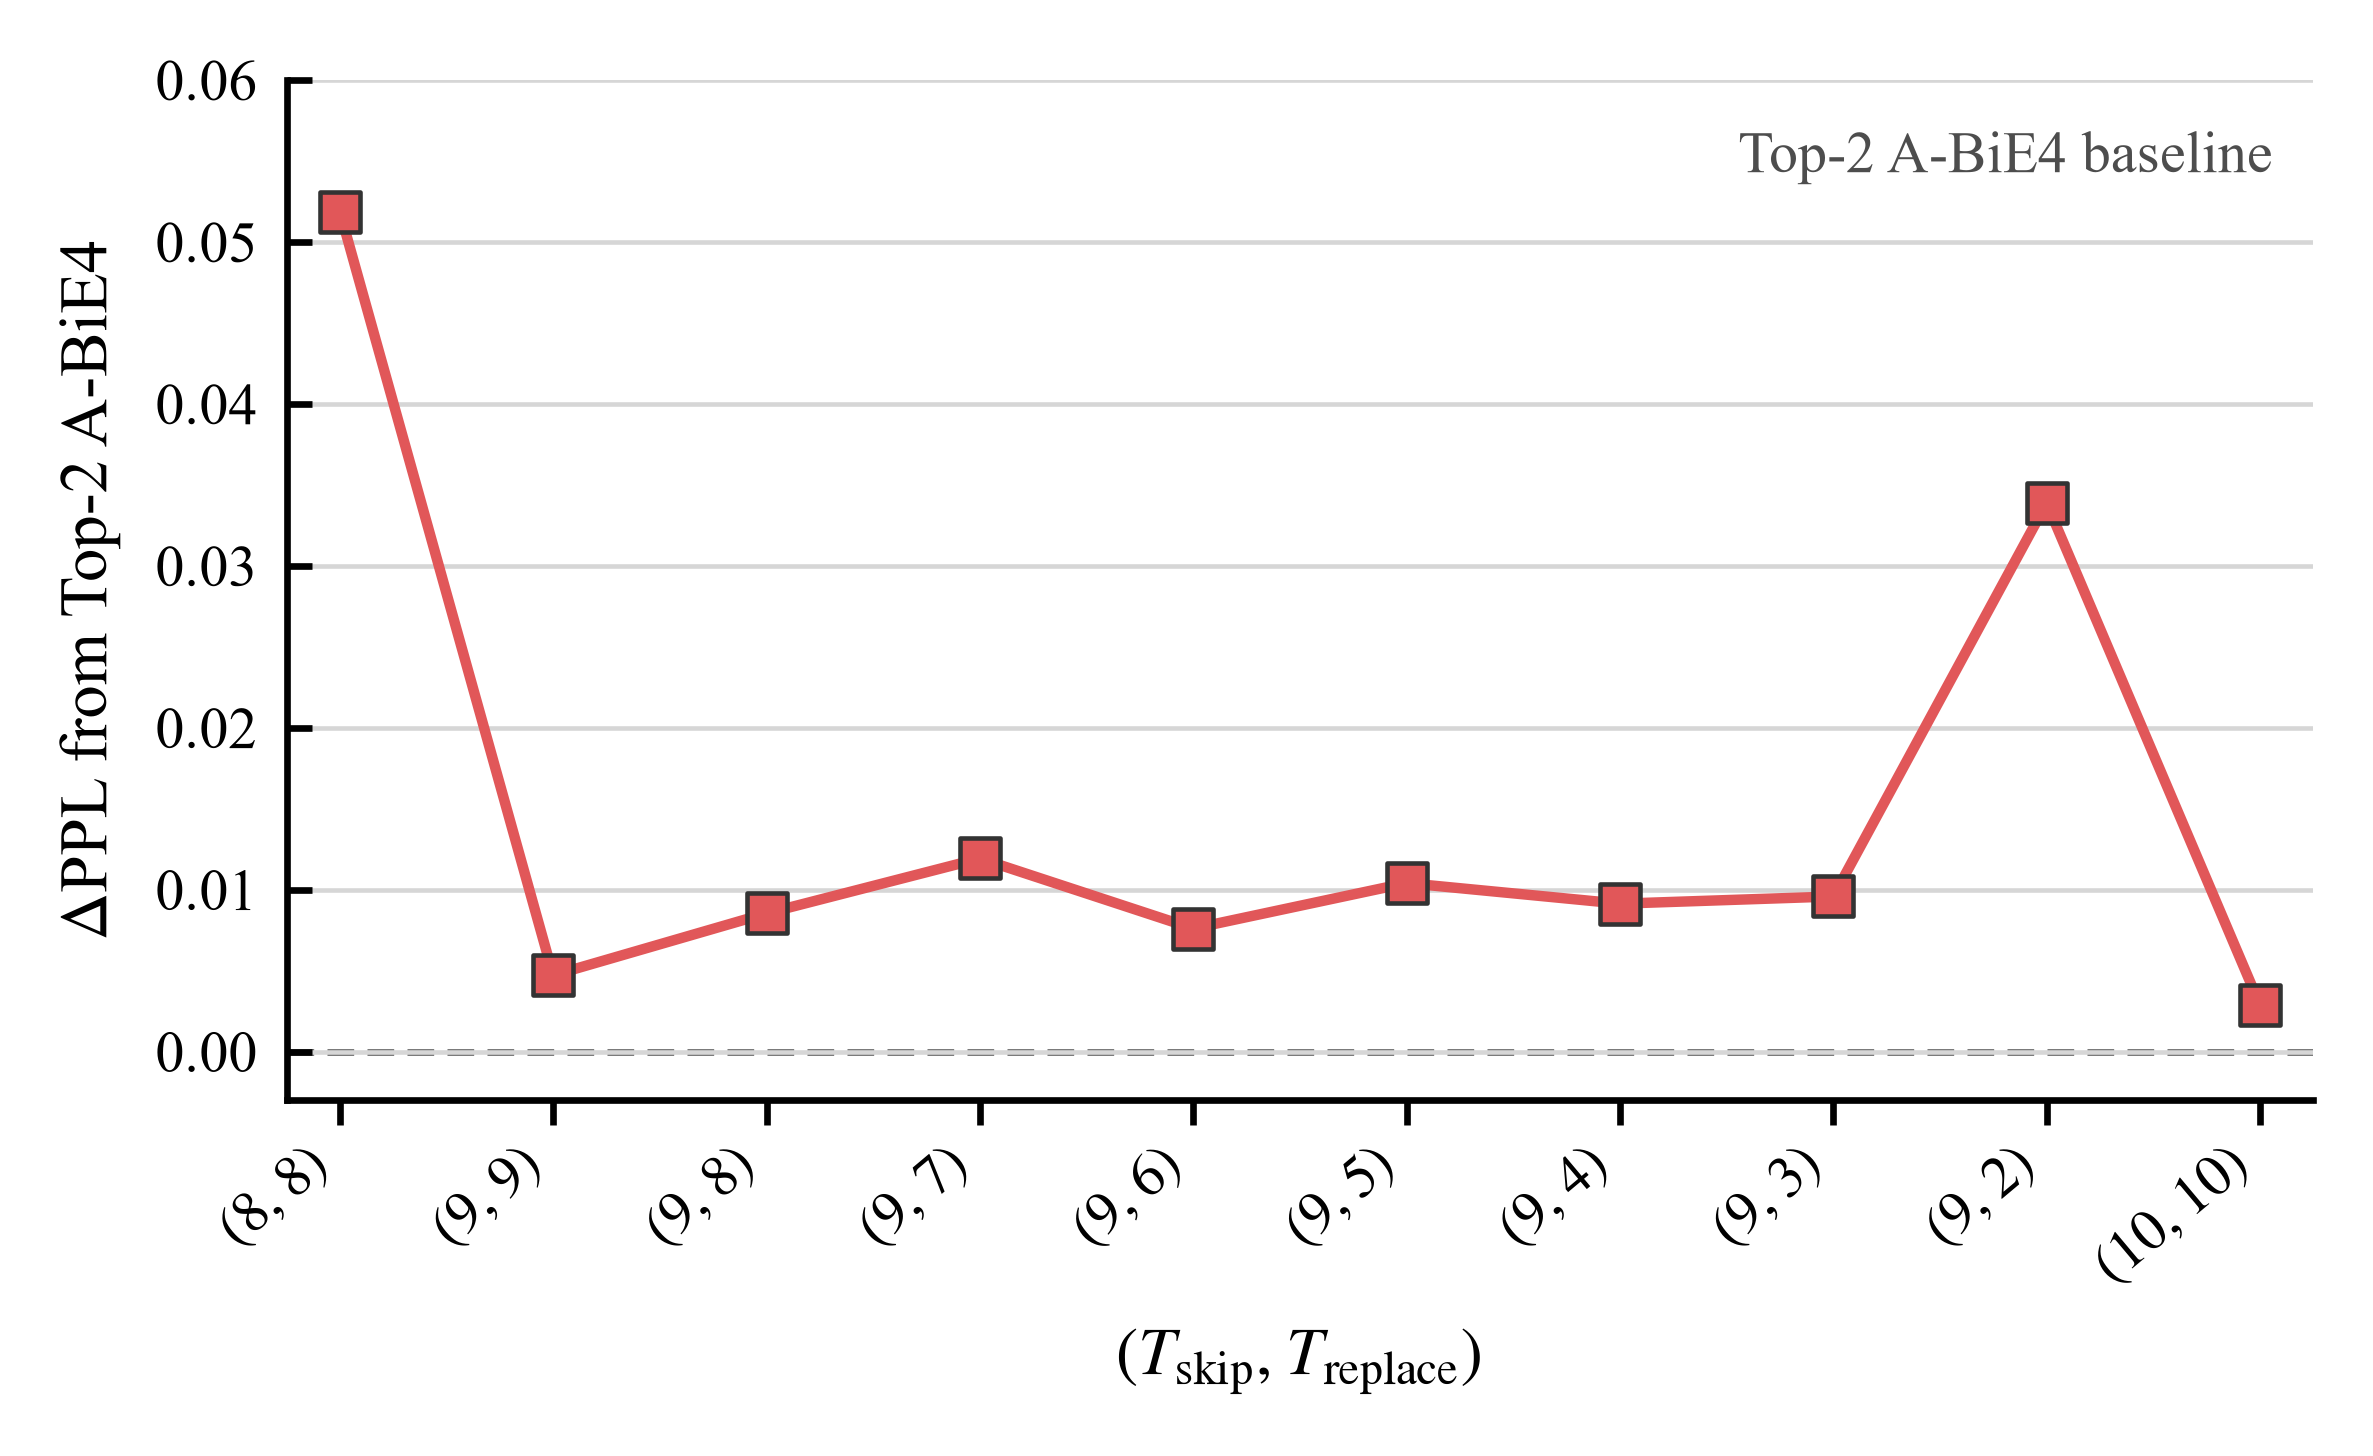
\includegraphics[width=\linewidth]{figures/fig_hybrid_sweep.png}
    \caption{Perplexity delta versus Top-2 baseline under asymmetric DEWA ($T_{\mathrm{skip}}$, $T_{\mathrm{replace}}$).}
    \label{fig:hybrid_sweep}
\end{figure}

\subsection{Hardware-Oriented Metrics}
Functional simulation reports DEWA out-of-window (OOW) decisions and optimistic FP-Acc request counts.
RTL synthesis of the baseline BFP-PE confirms FP-Acc dominance (Fig.~\ref{fig:bfp_pe_ppa}); synthesized area and power for the full Top-2 DEWA design remain future work.
